
\begin{figure}[h!]
    \centering
    \caption{Distribution of share of workers who work where they live, 2017}
    \label{fig:shares_own_geo}
    \begin{subfigure}{.7\textwidth}
        \caption{ZIP code}
        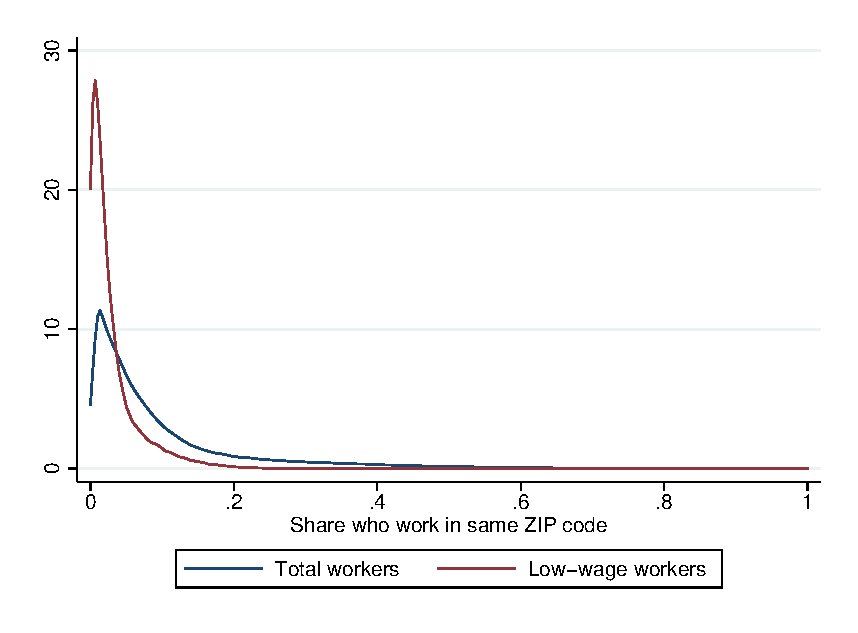
\includegraphics[width = \textwidth]
            {descriptive/shares/output/shares_zipcode}
    \end{subfigure}\\
    \begin{subfigure}{.7\textwidth}
        \caption{County}
        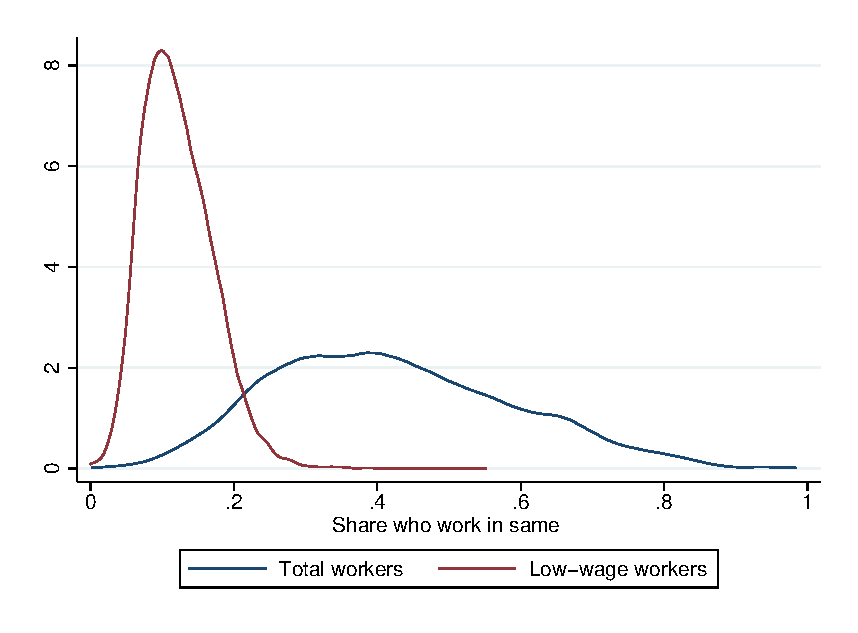
\includegraphics[width = \textwidth]
            {descriptive/shares/output/shares_county}
    \end{subfigure}

    \begin{minipage}{.95\textwidth} \footnotesize
        \vspace{3mm}
        \textit{Notes:} 
        Data are from LODES origin-destination matrices \parencite{LODES}, 
        aggregated at the ZIP code and county levels.
        The figure shows the estimated distribution of the share of workers who 
        reside and work in the same geographical unit, at the ZIP code (panel a)
        and County (panel b) levels.
    \end{minipage}
\end{figure}

\clearpage
\begin{figure}[h!]
    \centering
    \caption{Distribution of Minimum Wage Changes}
    \label{fig:d_ln_mw_dist}
    \begin{subfigure}{.7\textwidth}
        \caption{Intensity}
        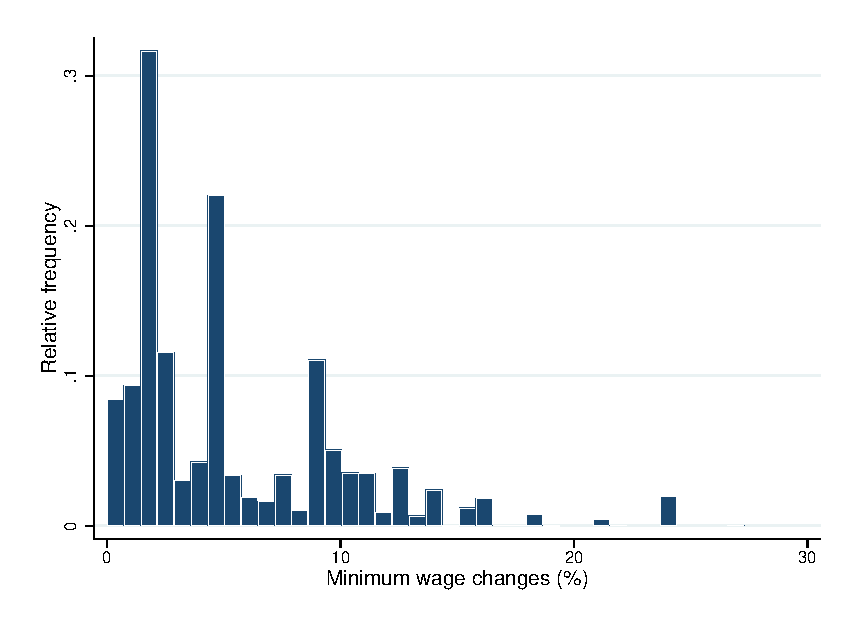
\includegraphics[width = \textwidth]
            {descriptive/desc_tables/output/pct_ch_mw_dist}
    \end{subfigure}\\
    \begin{subfigure}{.7\textwidth}
        \caption{Timing}
        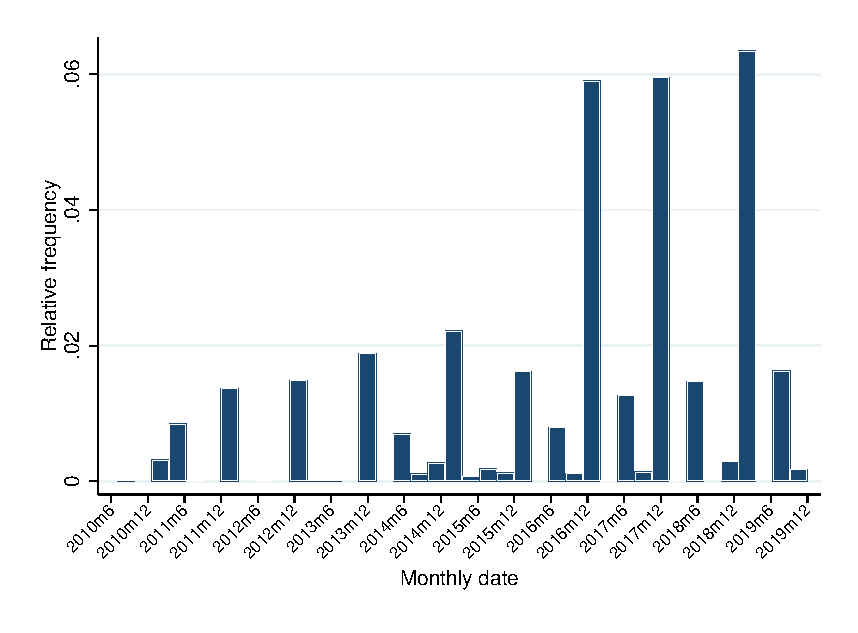
\includegraphics[width = \textwidth]
            {descriptive/desc_tables/output/pct_ch_mw_date_dist}
    \end{subfigure}

    \begin{minipage}{.95\textwidth} \footnotesize
        \vspace{3mm}
        \textit{Notes:} The histograms show the distribution of positive MW changes 
        in the full sample of ZIP codes available in the Zillow data. Panel (a) reports 
        the intensity of the changes in percentage terms. Panel (b) plots the distribution 
        across time of such changes. 
    \end{minipage}
\end{figure}

